% !TEX program = xelatex
% 计算物理 第一次作业报告
\RequirePackage{expl3}
\ExplSyntaxOn
\msg_redirect_name:nnn { fontspec } { no-script } { info }
\ExplSyntaxOff
\documentclass[UTF8,a4paper,12pt]{ctexart}

\usepackage{amsmath,amssymb}
\usepackage{graphicx}
\usepackage{geometry}
\usepackage{listings}
\usepackage{xcolor}
\usepackage{float}
\usepackage{fancyhdr}
\usepackage{hyperref}

\geometry{margin=2.5cm}
\graphicspath{{imgs/}}
\hypersetup{colorlinks=true,linkcolor=blue,urlcolor=blue}

% 页码居中置于页面底部
\pagestyle{fancy}
\fancyhf{}
\fancyfoot[C]{\thepage}
\renewcommand{\headrulewidth}{0pt}
\renewcommand{\footrulewidth}{0pt}

% 章节序号用中文：一、 二、 （一）（二）
% aftername 控制序号与标题文字之间的间距，置空以缩短间隔
\ctexset{
  section/number       = \chinese{section},
  section/name         = {,、},
  section/aftername    = {},
  subsection/number    = \chinese{subsection},
  subsection/name      = {（,）},
  subsection/aftername = {},
}

\lstset{
  basicstyle=\ttfamily\small,
  breaklines=true,
  frame=single,
  numbers=left,
  numberstyle=\tiny\color{gray},
  keywordstyle=\color{blue!70!black},
  commentstyle=\color{green!45!black},
  stringstyle=\color{red!60!black},
  showstringspaces=false,
  columns=flexible,
  language=Python,
}

\title{第一次作业——简谐振动的合成与李萨如图形}
\author{课程名称：计算物理\quad 授课教师：靳亚康\\[0.2em]专业：应用物理\quad 姓名：刘越\quad 学号：2024120101019}
\date{\today}

\begin{document}
\maketitle

% =====================================================================
\section{题目解析}

\subsection{题目背景}

一维简谐振动的一般形式可以写成
\begin{equation}
  x = A\sin(\omega t + \varphi_0),
\end{equation}
其中 $A$ 是振幅，$\omega$ 是角频率，$\varphi_0$ 是初相位。题目把它推广到二维：在 $x$、$y$ 两个相互垂直的方向上各放一个简谐振动，
\begin{equation}
  x = 3\sin(3t),\qquad y = 3\sin\!\left(3t + \frac{\pi}{6}\right).
\end{equation}
两个方向的振幅均为 $A=3$，角频率均为 $\omega=3$，唯一的差别是 $x$、$y$ 之间存在相位差 $\Delta\varphi=\pi/6$。要研究的就是这样一个“二维振子”在 $x$-$y$ 平面上画出来的轨迹。

\subsection{任务拆解}

题目的三条要求：

\begin{enumerate}
  \item 编写 Python 程序，把上述振动在时间轴上离散取样，得到每个时刻的 $(x,y)$ 坐标；
  \item 把取样点连起来画在 $x$-$y$ 平面上，即振动轨迹；
  \item 改变振动参数，观察并分析轨迹的变化规律，并加以讨论。
\end{enumerate}

前两条属于实现，第三条是重点，其核心在于判断：这几个参数中，哪一个决定图形的\textbf{形状}，哪一个决定它的\textbf{取向}与\textbf{宽窄}，以及各自对应的物理意义。

\subsection{先行解析推导}

编程之前，先将两个方程联立，作一次解析推导，以作为检验数值结果的参照。记相位差 $\delta=\Delta\varphi=\pi/6$。由 $x=A\sin\omega t$ 得
\[
  \sin\omega t=\frac{x}{A},\qquad
  \cos\omega t=\pm\sqrt{1-\frac{x^{2}}{A^{2}}} .
\]
把它代进 $y$ 的表达式：
\[
  y=A\sin(\omega t+\delta)
  =A\big(\sin\omega t\cos\delta+\cos\omega t\sin\delta\big)
  =x\cos\delta+\sin\delta\sqrt{A^{2}-x^{2}} .
\]
移项、两边平方、再整理：
\[
  (y-x\cos\delta)^{2}=\sin^{2}\delta\,\big(A^{2}-x^{2}\big)
  \;\Longrightarrow\;
  x^{2}+y^{2}-2xy\cos\delta = A^{2}\sin^{2}\delta .
\]
这就是两个同频正交简谐振动合成的轨迹方程。把 $A=3$、$\delta=\pi/6$（$\cos\delta=\tfrac{\sqrt3}{2}$，$\sin^{2}\delta=\tfrac14$）代进去：
\begin{equation}
  \boxed{\,x^{2}+y^{2}-\sqrt{3}\,xy=\frac{9}{4}\,}
\end{equation}
这是一个主轴相对于坐标轴旋转了 $45^\circ$ 的椭圆。程序输出应当与该式吻合，若不符则说明程序存在错误。有了这个式子，后面讨论“参数变化”时就有了可以对照的解析依据。

% =====================================================================
\section{算法}

\subsection{数值离散化}

简谐振动是连续函数，但计算机只能处理有限个点，因此需要把时间轴离散化。做法是用 \texttt{numpy} 把时间轴离散成 $N$ 个等间距的点：

\begin{lstlisting}
t = np.linspace(0, 2*np.pi, 10000)
\end{lstlisting}

其中有两点值得说明：

\begin{itemize}
  \item \textbf{区间取 $[0,2\pi]$。} 因为 $\omega=3$，相位 $3t$ 在 $t\in[0,2\pi]$ 里恰好走过 $3$ 个完整周期，回到出发点，所以轨迹是闭合的。区间不取整周期时，曲线会缺少一段，图形不完整。
  \item \textbf{取 $N=10000$。} 取样点过少时，弧线会被画成一节一节的折线；点足够密，曲线才平滑。该取值不影响物理结论，但影响图像的显示效果。
\end{itemize}

\subsection{参数扫描设计}

第 3 条要求“改变振动参数”。可调参数有三个：振幅 $A$、角频率 $\omega$（更本质地是频率比 $\omega_x:\omega_y$）、相位差 $\Delta\varphi$。为单独分析各个参数的作用，采用\textbf{控制变量法}，每次只改变一个参数，固定其余两个：

\begin{enumerate}
  \item 固定 $A=3$、$\omega=3$，令相位差取 $\Delta\varphi = 0,\ \pi/6,\ \pi/2$；
  \item 固定 $A=3$、$\Delta\varphi=0$，令频率比取 $1{:}1,\ 3{:}4,\ 1{:}2$；
  \item 固定 $\omega_x=\omega_y=3$、$\Delta\varphi=\pi/6$，令振幅比取 $(A_x,A_y)=(3,3),(3,1),(1,3)$。
\end{enumerate}

三组各绘制为一张三联图，便于逐项对比各参数的作用。

\subsection{绘图注意事项}

绘制时需注意：\texttt{matplotlib} 默认会按画布比例自动缩放两个坐标轴，纵横比例不一致时，圆会被压成椭圆、椭圆也会被拉变形。因此必须加一句

\begin{lstlisting}
ax.axis('equal')
\end{lstlisting}

以强制 $x$、$y$ 采用相同的单位长度。后续所有讨论都建立在“图形没有失真”这一前提上，该步骤不可省略。

\subsection{核心代码}

原题轨迹的绘制（对应 \texttt{hw1\_t1.py}，此处节选关键几行）：

\begin{lstlisting}[caption={简谐振动轨迹的绘制（hw1\_t1.py 节选）}]
import numpy as np
import matplotlib.pyplot as plt

# Sample the time axis over exactly one closing period
t = np.linspace(0, 2*np.pi, 10000)

# Two perpendicular simple harmonic vibrations
x = 3 * np.sin(3 * t)
y = 3 * np.sin(3 * t + np.pi/6)

plt.plot(x, y)
plt.axis('equal')      # keep the true aspect ratio, avoid distortion
plt.grid(True)
plt.show()
\end{lstlisting}

参数扫描部分（对应 \texttt{hw1\_t2.py}，用三组 \texttt{subplots} 各绘制一张三联图）：

\begin{lstlisting}[caption={参数扫描：相位差、频率比、振幅比（hw1\_t2.py 节选）}]
# Case 1: sweep the phase difference (A and omega fixed)
for dphi in [0, np.pi/6, np.pi/2]:
    x = 3*np.sin(3*t)
    y = 3*np.sin(3*t + dphi)

# Case 2: sweep the frequency ratio (phase difference = 0 fixed)
for wx, wy in [(3,3), (3,4), (3,6)]:
    x = 3*np.sin(wx*t)
    y = 3*np.sin(wy*t)

# Case 3: sweep the amplitude ratio (omega = 3, phase difference = pi/6)
for Ax, Ay in [(3,3), (3,1), (1,3)]:
    x = Ax*np.sin(3*t)
    y = Ay*np.sin(3*t + np.pi/6)
\end{lstlisting}

程序采用向量化运算，没有显式循环，时间复杂度为 $O(N)$。

% =====================================================================
\section{结果讨论}

本节按题目第 3 条展开：改变参数、观察变化、分析讨论。

\subsection{原题轨迹：倾斜椭圆}

图 \ref{fig:t1} 是题目给定参数（$A=3$，$\omega=3$，$\Delta\varphi=\pi/6$）下的轨迹。

\begin{figure}[H]
  \centering
  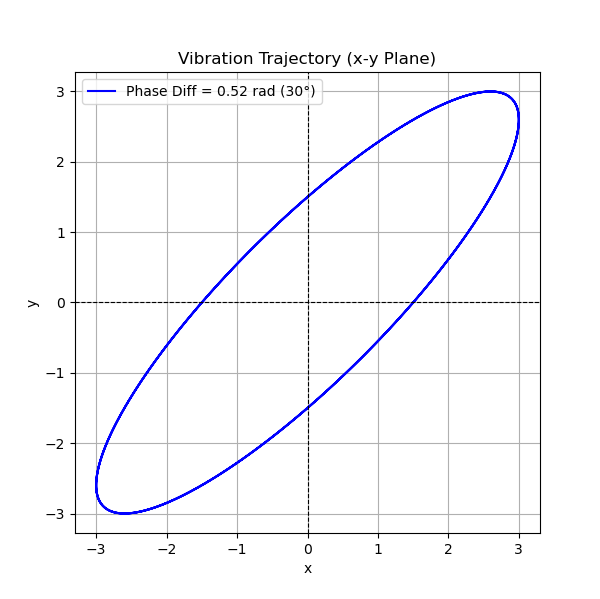
\includegraphics[width=0.55\textwidth]{t1.png}
  \caption{原题参数下的振动轨迹（$A=3$，$\omega=3$，$\Delta\varphi=\pi/6$）。}
  \label{fig:t1}
\end{figure}

该轨迹是一条倾斜的椭圆，长轴大致沿着 $y=x$ 方向，与第一节推导所得的轨迹方程 $x^{2}+y^{2}-\sqrt3\,xy=\tfrac94$ 完全吻合。

进一步计算椭圆的长短轴。令 $u=\dfrac{x+y}{\sqrt2}$、$v=\dfrac{x-y}{\sqrt2}$（相当于把坐标轴转到 $45^\circ$ 方向），代入后椭圆变成标准形式
\[
  u^{2}\Big(1-\frac{\sqrt3}{2}\Big)+v^{2}\Big(1+\frac{\sqrt3}{2}\Big)=\frac94
  \;\Longrightarrow\;
  \frac{u^{2}}{a^{2}}+\frac{v^{2}}{b^{2}}=1,
\]
其中 $a\approx 4.10$（沿 $u$ 方向，即 $y=x$），$b\approx 1.10$（沿 $v$ 方向，即 $y=-x$），长短轴之比约为 $3.7$。

其次判断旋转方向。在 $t=0$ 时刻，质点位于 $(0,\,1.5)$，速度为 $(9\cos0,\ 9\cos\tfrac{\pi}{6})=(9,\ 7.79)$，指向第一象限；质点由 $y$ 轴正方向转向 $x$ 轴正方向，故轨迹为\textbf{顺时针}方向。这印证了一条规律：当 $y$ 的相位\textbf{超前} $x$（此处 $\delta>0$）时，旋转方向为顺时针；反之则为逆时针。

物理上，这是“两个正交简谐振动合成”最基本的结果：相位差既不为 $0$ 也不为 $\pi/2$ 时，轨迹就是一个椭圆。

\subsection{相位差的影响}

图 \ref{fig:phase} 固定振幅和频率，只改变相位差，取 $\Delta\varphi=0,\ \pi/6,\ \pi/2$。

\begin{figure}[H]
  \centering
  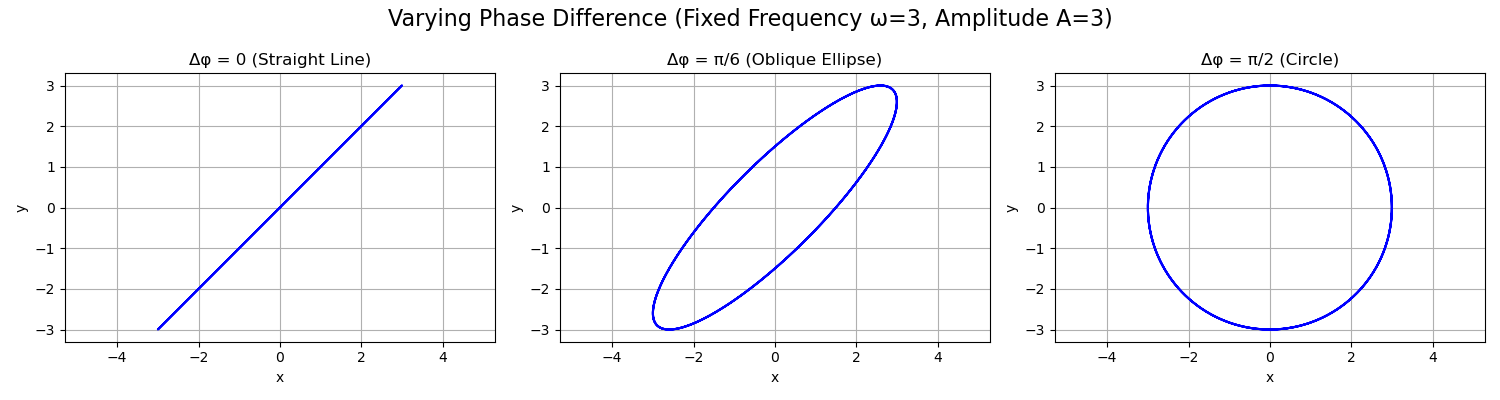
\includegraphics[width=0.98\textwidth]{t2_1.png}
  \caption{固定 $A=3$、$\omega=3$，只改变相位差。}
  \label{fig:phase}
\end{figure}

\begin{itemize}
  \item \textbf{$\Delta\varphi=0$：} 两个振动步调完全一致，$x\equiv y$，轨迹退化成一条直线 $y=x$（斜率等于振幅比 $A_y/A_x=1$），质点沿这条直线往复振动。
  \item \textbf{$\Delta\varphi=\pi/6$：} 即原题的斜椭圆，与直线相比已明显张开。
  \item \textbf{$\Delta\varphi=\pi/2$：} 等振幅条件下，轨迹变成一个\textbf{正圆}。把 $A=3$、$\cos\delta=0$、$\sin^2\delta=1$ 代入轨迹方程，得到 $x^{2}+y^{2}=9$，半径为 $3$。
\end{itemize}

由此可见，相位差控制椭圆的“张开程度”：从 $0$ 增至 $\pi/2$，轨迹由压扁的直线逐渐张开成圆。此处可得一个简洁的结论——\textbf{匀速圆周运动等价于两个同频、等幅、相位差为 $\pi/2$ 的正交简谐振动之和}；而一般椭圆则是介于直线与圆之间的运动。

这一结果与光学中的偏振态图像一致：两个同频、振动方向互相垂直的光振动叠加时，合成光的偏振态由相位差与振幅比共同决定——$\Delta\varphi=0$ 或 $\pi$ 对应\textbf{线偏振}，$\Delta\varphi=\pm\pi/2$ 且等振幅对应\textbf{圆偏振}，其余情形为\textbf{椭圆偏振}。

\subsection{频率比的影响}

图 \ref{fig:freq} 固定振幅和相位差（$\Delta\varphi=0$），改变频率比 $\omega_x:\omega_y = 1{:}1,\ 3{:}4,\ 1{:}2$。

\begin{figure}[H]
  \centering
  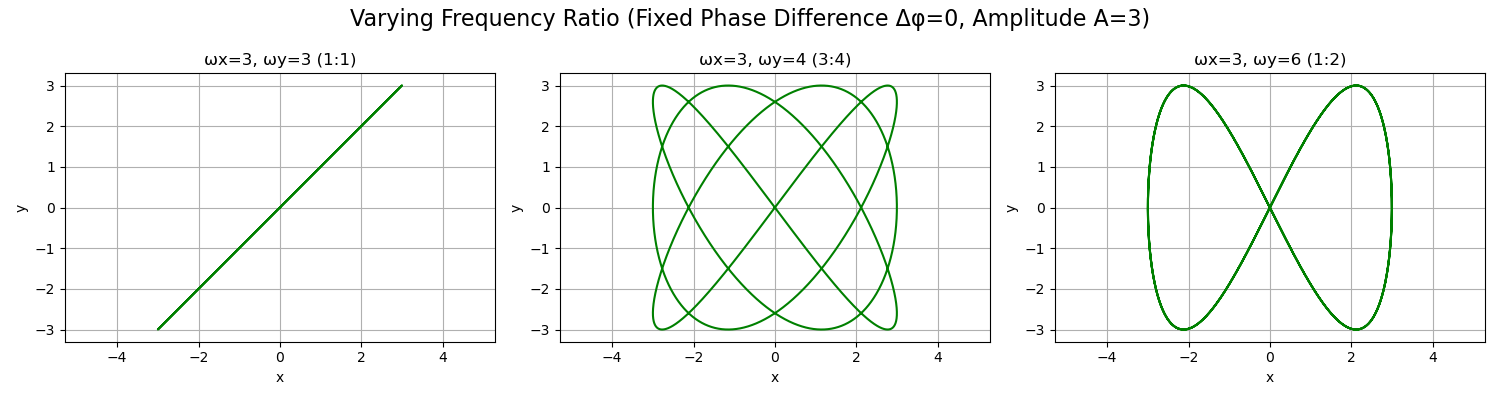
\includegraphics[width=0.98\textwidth]{t2_2.png}
  \caption{固定 $A=3$、$\Delta\varphi=0$，只改变频率比。}
  \label{fig:freq}
\end{figure}

\begin{itemize}
  \item \textbf{$1{:}1$：} 由于 $\Delta\varphi=0$，退化成直线 $y=x$；
  \item \textbf{$3{:}4$：} 出现典型的李萨如图形，曲线在竖直边 $x=\pm3$ 上相切 $3$ 次，在水平边 $y=\pm3$ 上相切 $4$ 次；
  \item \textbf{$1{:}2$：} 图形结构更为简单，竖直边相切 $1$ 次、水平边相切 $2$ 次。
\end{itemize}

由此可归纳出清晰的规律：把频率比化成最简整数比 $p:q$ 后，轨迹是闭合的，且与竖直边（$x$ 方向）的切点数恰好是 $p$，与水平边的切点数恰好是 $q$，也就是\textbf{切点数之比等于频率比}。

物理意义上，\textbf{频率比决定轨迹的拓扑结构}：只要两个频率之比是有理数，运动就是严格周期的，轨迹闭合为规则的花纹；而如果频率之比是无理数，两次振动始终无法对齐，曲线不会闭合，而会越画越密，最终稠密地铺满整个矩形区域。该规律在实验中也有直接应用：把两个待测信号分别接入示波器的 X、Y 通道，统计切点数即可读出频率比，这正是\textbf{李萨如法测频率}的原理。

\subsection{振幅比的影响}

图 \ref{fig:amp} 固定频率比 $1{:}1$ 和相位差 $\pi/6$，只改变振幅比。

\begin{figure}[H]
  \centering
  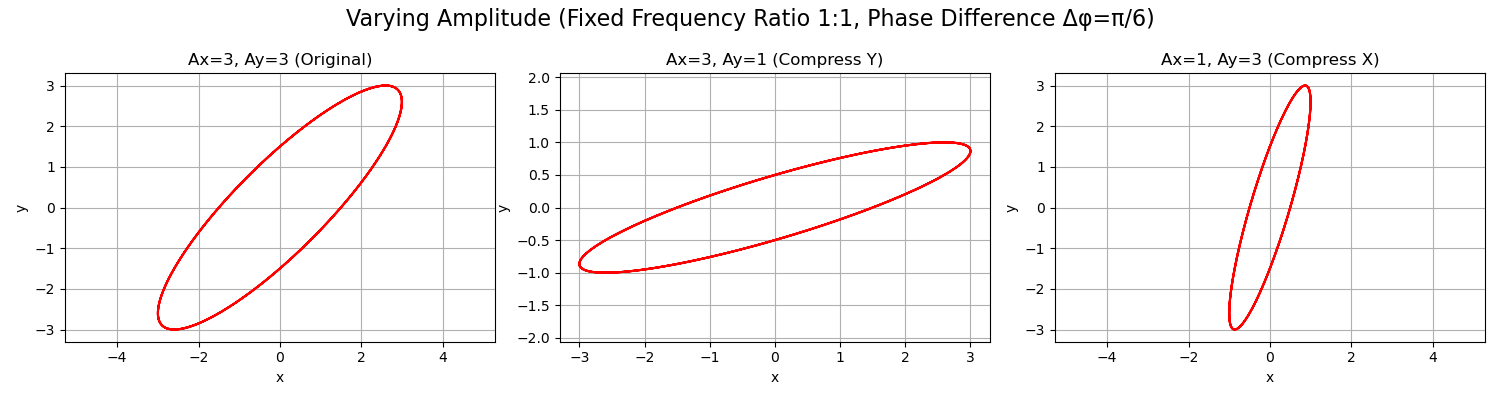
\includegraphics[width=0.98\textwidth]{t2_3.png}
  \caption{固定 $\omega_x=\omega_y=3$、$\Delta\varphi=\pi/6$，只改变振幅比。}
  \label{fig:amp}
\end{figure}

\begin{itemize}
  \item \textbf{$(A_x,A_y)=(3,3)$：} 原椭圆；
  \item \textbf{$(3,1)$：} $y$ 方向的振幅减小，椭圆趋于扁平并贴着 $x$ 轴；
  \item \textbf{$(1,3)$：} 反之，$x$ 方向的振幅减小，椭圆趋于竖直。
\end{itemize}

综上，改变振幅比相当于对图形作一次\textbf{各向异性缩放}：它只改变轨迹的包围矩形尺寸 $2A_x\times 2A_y$，即把图形压扁或拉长，但\textbf{不改变曲线是否闭合，也不改变旋转方向}——闭合性与转向由频率比和相位差的符号决定。

结合上一小节还可得到一个更完整的结论：轨迹要成为\textbf{正圆}，必须同时满足两个条件——相位差为 $\pi/2$ \emph{且} 振幅相等，只满足其中一个，得到的都是椭圆。这对应光学中椭圆偏振光的“椭圆度”：它由两个分量的振幅比和相位差共同决定，缺一不可。

\subsection{三个参数的作用}

把上述结果汇总如下：

\begin{table}[H]
  \centering
  \caption{三个参数对轨迹的影响}
  \begin{tabular}{|p{3.2cm}|p{5.0cm}|p{5.4cm}|}
    \hline
    参数                       & 决定什么                       & 极端情形                                            \\
    \hline
    相位差 $\Delta\varphi$     & 轨迹的形状类型与“张开程度”     & $\Delta\varphi=0$ 退化为直线；$=\pi/2$ 且等幅时为圆 \\
    \hline
    频率比 $\omega_x:\omega_y$ & 轨迹的拓扑（是否闭合、多少瓣） & 有理比闭合；无理比不闭合                            \\
    \hline
    振幅比 $A_x:A_y$           & 各方向尺度（“宽窄”）           & 等幅且 $\Delta\varphi=\pi/2$ 时为圆                 \\
    \hline
  \end{tabular}
\end{table}

统一地看，一般椭圆的轨迹方程是
\begin{equation}
  \frac{x^{2}}{A_x^{2}}+\frac{y^{2}}{A_y^{2}}-\frac{2xy\cos\delta}{A_x A_y}=\sin^{2}\delta ,
\end{equation}
三个参数即由这一个式子抽出的三个可变参量。

上述结论在物理中有广泛的应用：除了前面提到的\textbf{偏振光}和\textbf{示波器李萨如测频}，还有\textbf{分子与晶格振动}（耦合的简正模式在小振动下常表现为两个方向的简谐振动叠加）以及\textbf{二自由度系统}（质点在二维势阱中的小振动）。

% =====================================================================
\section{AI使用说明}

本报告在撰写过程中使用人工智能工具（Claude Code + DeepSeek-4.1-Flash）辅助完成，具体用途如下：

\begin{enumerate}
  \item \textbf{撰写报告标题大纲。} 借助 AI 拟定报告的整体框架，在“题目解析—算法—结果讨论”的三节结构上细分，并梳理各节的标题与内容要点。
  \item \textbf{LaTeX 图文排版。} 借助 AI 完成 LaTeX 源文件的编写与排版，包括公式录入、结果图的插入与尺寸设置、表格绘制，以及页眉页脚、章节序号等版式调整。
  \item \textbf{物理结论检查。} 借助 AI 复核报告中的物理结论，包括轨迹方程的推导、椭圆长短轴与旋转方向的判断、以及频率比与切点数关系的验证，并对关键结论作数值校验。
\end{enumerate}

以上即 AI 在本报告中的全部用途。

\end{document}
